% Options for packages loaded elsewhere
\PassOptionsToPackage{unicode}{hyperref}
\PassOptionsToPackage{hyphens}{url}
\PassOptionsToPackage{dvipsnames,svgnames,x11names}{xcolor}
%
\documentclass[
  letterpaper,
  DIV=11,
  numbers=noendperiod]{scrreprt}

\usepackage{amsmath,amssymb}
\usepackage{iftex}
\ifPDFTeX
  \usepackage[T1]{fontenc}
  \usepackage[utf8]{inputenc}
  \usepackage{textcomp} % provide euro and other symbols
\else % if luatex or xetex
  \usepackage{unicode-math}
  \defaultfontfeatures{Scale=MatchLowercase}
  \defaultfontfeatures[\rmfamily]{Ligatures=TeX,Scale=1}
\fi
\usepackage{lmodern}
\ifPDFTeX\else  
    % xetex/luatex font selection
\fi
% Use upquote if available, for straight quotes in verbatim environments
\IfFileExists{upquote.sty}{\usepackage{upquote}}{}
\IfFileExists{microtype.sty}{% use microtype if available
  \usepackage[]{microtype}
  \UseMicrotypeSet[protrusion]{basicmath} % disable protrusion for tt fonts
}{}
\makeatletter
\@ifundefined{KOMAClassName}{% if non-KOMA class
  \IfFileExists{parskip.sty}{%
    \usepackage{parskip}
  }{% else
    \setlength{\parindent}{0pt}
    \setlength{\parskip}{6pt plus 2pt minus 1pt}}
}{% if KOMA class
  \KOMAoptions{parskip=half}}
\makeatother
\usepackage{xcolor}
\setlength{\emergencystretch}{3em} % prevent overfull lines
\setcounter{secnumdepth}{5}
% Make \paragraph and \subparagraph free-standing
\ifx\paragraph\undefined\else
  \let\oldparagraph\paragraph
  \renewcommand{\paragraph}[1]{\oldparagraph{#1}\mbox{}}
\fi
\ifx\subparagraph\undefined\else
  \let\oldsubparagraph\subparagraph
  \renewcommand{\subparagraph}[1]{\oldsubparagraph{#1}\mbox{}}
\fi


\providecommand{\tightlist}{%
  \setlength{\itemsep}{0pt}\setlength{\parskip}{0pt}}\usepackage{longtable,booktabs,array}
\usepackage{calc} % for calculating minipage widths
% Correct order of tables after \paragraph or \subparagraph
\usepackage{etoolbox}
\makeatletter
\patchcmd\longtable{\par}{\if@noskipsec\mbox{}\fi\par}{}{}
\makeatother
% Allow footnotes in longtable head/foot
\IfFileExists{footnotehyper.sty}{\usepackage{footnotehyper}}{\usepackage{footnote}}
\makesavenoteenv{longtable}
\usepackage{graphicx}
\makeatletter
\def\maxwidth{\ifdim\Gin@nat@width>\linewidth\linewidth\else\Gin@nat@width\fi}
\def\maxheight{\ifdim\Gin@nat@height>\textheight\textheight\else\Gin@nat@height\fi}
\makeatother
% Scale images if necessary, so that they will not overflow the page
% margins by default, and it is still possible to overwrite the defaults
% using explicit options in \includegraphics[width, height, ...]{}
\setkeys{Gin}{width=\maxwidth,height=\maxheight,keepaspectratio}
% Set default figure placement to htbp
\makeatletter
\def\fps@figure{htbp}
\makeatother

\KOMAoption{captions}{tableheading}
\makeatletter
\@ifpackageloaded{tcolorbox}{}{\usepackage[skins,breakable]{tcolorbox}}
\@ifpackageloaded{fontawesome5}{}{\usepackage{fontawesome5}}
\definecolor{quarto-callout-color}{HTML}{909090}
\definecolor{quarto-callout-note-color}{HTML}{0758E5}
\definecolor{quarto-callout-important-color}{HTML}{CC1914}
\definecolor{quarto-callout-warning-color}{HTML}{EB9113}
\definecolor{quarto-callout-tip-color}{HTML}{00A047}
\definecolor{quarto-callout-caution-color}{HTML}{FC5300}
\definecolor{quarto-callout-color-frame}{HTML}{acacac}
\definecolor{quarto-callout-note-color-frame}{HTML}{4582ec}
\definecolor{quarto-callout-important-color-frame}{HTML}{d9534f}
\definecolor{quarto-callout-warning-color-frame}{HTML}{f0ad4e}
\definecolor{quarto-callout-tip-color-frame}{HTML}{02b875}
\definecolor{quarto-callout-caution-color-frame}{HTML}{fd7e14}
\makeatother
\makeatletter
\makeatother
\makeatletter
\@ifpackageloaded{bookmark}{}{\usepackage{bookmark}}
\makeatother
\makeatletter
\@ifpackageloaded{caption}{}{\usepackage{caption}}
\AtBeginDocument{%
\ifdefined\contentsname
  \renewcommand*\contentsname{Table of contents}
\else
  \newcommand\contentsname{Table of contents}
\fi
\ifdefined\listfigurename
  \renewcommand*\listfigurename{List of Figures}
\else
  \newcommand\listfigurename{List of Figures}
\fi
\ifdefined\listtablename
  \renewcommand*\listtablename{List of Tables}
\else
  \newcommand\listtablename{List of Tables}
\fi
\ifdefined\figurename
  \renewcommand*\figurename{Figure}
\else
  \newcommand\figurename{Figure}
\fi
\ifdefined\tablename
  \renewcommand*\tablename{Table}
\else
  \newcommand\tablename{Table}
\fi
}
\@ifpackageloaded{float}{}{\usepackage{float}}
\floatstyle{ruled}
\@ifundefined{c@chapter}{\newfloat{codelisting}{h}{lop}}{\newfloat{codelisting}{h}{lop}[chapter]}
\floatname{codelisting}{Listing}
\newcommand*\listoflistings{\listof{codelisting}{List of Listings}}
\makeatother
\makeatletter
\@ifpackageloaded{caption}{}{\usepackage{caption}}
\@ifpackageloaded{subcaption}{}{\usepackage{subcaption}}
\makeatother
\makeatletter
\@ifpackageloaded{tcolorbox}{}{\usepackage[skins,breakable]{tcolorbox}}
\makeatother
\makeatletter
\@ifundefined{shadecolor}{\definecolor{shadecolor}{rgb}{.97, .97, .97}}
\makeatother
\makeatletter
\makeatother
\makeatletter
\makeatother
\ifLuaTeX
  \usepackage{selnolig}  % disable illegal ligatures
\fi
\IfFileExists{bookmark.sty}{\usepackage{bookmark}}{\usepackage{hyperref}}
\IfFileExists{xurl.sty}{\usepackage{xurl}}{} % add URL line breaks if available
\urlstyle{same} % disable monospaced font for URLs
\hypersetup{
  pdftitle={A Comprehensive Toolkit for WiFi Sensing: Decoding urban spaces},
  pdfauthor={Juhyeon Park},
  colorlinks=true,
  linkcolor={blue},
  filecolor={Maroon},
  citecolor={Blue},
  urlcolor={Blue},
  pdfcreator={LaTeX via pandoc}}

\title{A Comprehensive Toolkit for WiFi Sensing: Decoding urban spaces}
\author{Juhyeon Park}
\date{2023-06-23}

\begin{document}
\maketitle
\ifdefined\Shaded\renewenvironment{Shaded}{\begin{tcolorbox}[boxrule=0pt, interior hidden, borderline west={3pt}{0pt}{shadecolor}, enhanced, frame hidden, breakable, sharp corners]}{\end{tcolorbox}}\fi

\renewcommand*\contentsname{Table of contents}
{
\hypersetup{linkcolor=}
\setcounter{tocdepth}{2}
\tableofcontents
}
\bookmarksetup{startatroot}

\hypertarget{preface}{%
\chapter*{Preface}\label{preface}}
\addcontentsline{toc}{chapter}{Preface}

\markboth{Preface}{Preface}

This book is a dedicated resource for anyone interested in leveraging
affordable, commercially available sensors to measure non-motorized
traffic in urban environments.

Quantifying non-motorized traffic---such as pedestrians and
cyclists---plays a crucial role in urban studies. Understanding the flow
and patterns of non-motorized traffic can inform urban planning
strategies, enhance public safety, and contribute to the development of
sustainable cities. Moreover, sensing technologies provide a robust and
non-invasive method for capturing this vital information in real time,
offering insights that traditional surveys or manual counts might miss.

The advent of the Internet-of-Things (IoT) has spurred a wave of urban
sensing projects worldwide. Examples include the
\href{https://arrayofthings.github.io/}{Array of Things (AoT) in
Chicago, USA} and
\href{https://github.com/seoul-iotdata/S-DoT_SampleData}{S-DoT in Seoul,
Korea}, which utilize a network of sensors to gather a wide range of
data.

With the increasing accessibility of DIY technologies, individuals now
have the opportunity to engage with their urban environment in new and
innovative ways. These tools democratize the field of urban sensing,
previously the domain of expert scientists, by equipping anyone with the
interest to build their own sensors.

This book is designed for those interested in understanding and
monitoring non-motorized traffic. We provide comprehensive guidance on
building your own urban DIY sensors for this purpose. With hands-on
advice, practical examples, and detailed breakthroughs, our aim is to
empower you with the skills and knowledge necessary to contribute to the
rapidly evolving field of urban sensing.

\hypertarget{scope-of-this-document}{%
\subsection*{Scope of this document}\label{scope-of-this-document}}
\addcontentsline{toc}{subsection}{Scope of this document}

This document demonstrates 1) how to build a smart sensor that detects
pedestrians outdoors through WiFi sensing, and 2) how to analyze the
resulting data to produce meaningful insights. This includes:

\begin{itemize}
\tightlist
\item
  Getting
\item
  WiFi data preprocessing
\item
  WiFi data analysis
\end{itemize}

\hypertarget{why-wifi-sensing}{%
\subsection*{Why WiFi sensing?}\label{why-wifi-sensing}}
\addcontentsline{toc}{subsection}{Why WiFi sensing?}

WiFi sensing technologies are among these tools, providing a
non-invasive method for monitoring pedestrians outdoors via sensors that
detect WiFi packets sent regularly by access points (APs) and
WiFi-enabled devices. Most pedestrians today carry smart devices
equipped with WiFi network interfaces, and each WiFi packet includes
unique 48-bit addresses, known as Media Access Control (MAC) addresses,
enabling a device to be tracked by multiple WiFi sensors. Many recent
studies have utilized these sensing technologies to identify pedestrian
movements and behaviors\footnote{Duives, D. C., van Oijen, T., \&
  Hoogendoorn, S. P. (2020). Enhancing Crowd Monitoring System
  Functionality through Data Fusion: Estimating Flow Rate from Wi-Fi
  Traces and Automated Counting System Data. Sensors (Basel), 20(21).
  https://doi.org/10.3390/s20216032}\footnote{Soundararaj, B., Cheshire,
  J., \& Longley, P. (2019). Estimating real-time high-street footfall
  from Wi-Fi probe requests. International Journal of Geographical
  Information Science, 34(2), 325-343,.
  https://doi.org/10.1080/13658816.2019.1587616}\footnote{Zhou, Y., Lau,
  B. P. L., Koh, Z., Yuen, C., \& Ng, B. K. K. (2020). Understanding
  Crowd Behaviors in a Social Event by Passive WiFi Sensing and Data
  Mining. IEEE internet of things journal, 1-1,.
  https://doi.org/10.1109/jiot.2020.2972062}.

\bookmarksetup{startatroot}

\hypertarget{section}{%
\chapter{}\label{section}}

\part{2. Setting up WiFi Sensors}

\hypertarget{requirements}{%
\chapter*{2.1. Requirements}\label{requirements}}
\addcontentsline{toc}{chapter}{2.1. Requirements}

\markboth{2.1. Requirements}{2.1. Requirements}

\hypertarget{hardware-requirements}{%
\section*{2.1.1. Hardware Requirements}\label{hardware-requirements}}
\addcontentsline{toc}{section}{2.1.1. Hardware Requirements}

\markright{2.1.1. Hardware Requirements}

This is the hardware setup illustrating the necessary components
required for Wi-Fi sensing:

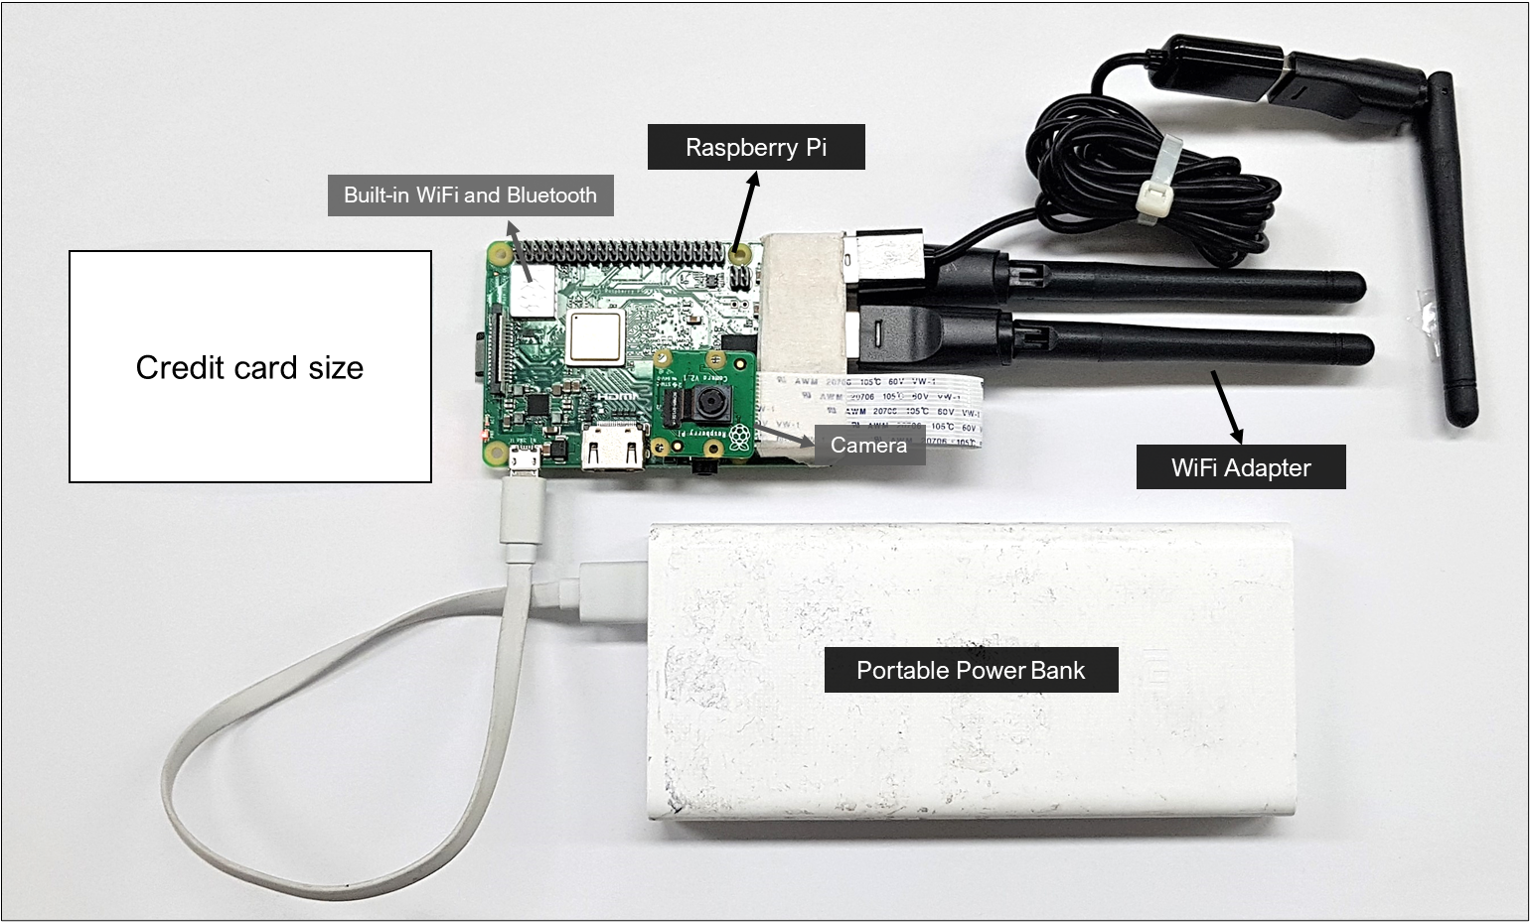
\includegraphics{content/material/ch2/sensor-comp.png}

To build up this WiFi sensor, you'll need the following hardware:

\begin{longtable}[]{@{}
  >{\raggedright\arraybackslash}p{(\columnwidth - 4\tabcolsep) * \real{0.2535}}
  >{\raggedright\arraybackslash}p{(\columnwidth - 4\tabcolsep) * \real{0.2535}}
  >{\raggedright\arraybackslash}p{(\columnwidth - 4\tabcolsep) * \real{0.4930}}@{}}
\toprule\noalign{}
\begin{minipage}[b]{\linewidth}\raggedright
Item
\end{minipage} & \begin{minipage}[b]{\linewidth}\raggedright
Function
\end{minipage} & \begin{minipage}[b]{\linewidth}\raggedright
Requirement
\end{minipage} \\
\midrule\noalign{}
\endhead
\bottomrule\noalign{}
\endlastfoot
Laptop and LAN cable & Accessing and controlling the sensor & \\
Raspberry Pi board & Building the sensor & Pi 3B/3B+ or a higher model
Pi \\
WiFi adapter & Capturing WiFi packets & Check chipset compatibility for
`monitoring mode'
\href{https://unix.stackexchange.com/questions/614984/supported-chipset-for-monitor-mode-and-packet-injection-in-kali-linux}{(here)} \\
Micro SD card and adapter & Building and storing data & At least 16 GB
size \\
Ethernet cable & Connecting the Pi to your laptop & \\
Portable power bank & Powering the sensor in outdoor environments &
Battery capacity: +20,000 mAh (lasts one day in our setting) \\
Pi camera & Recording the scene in front of the sensor & \\
\end{longtable}

\hypertarget{software}{%
\section*{2.1.2. Software}\label{software}}
\addcontentsline{toc}{section}{2.1.2. Software}

\markright{2.1.2. Software}

This is a list of the main programs needed to build a Wi-Fi sensor and
handle the sensor data. I will also provide the download link for each
step later.

\begin{longtable}[]{@{}
  >{\raggedright\arraybackslash}p{(\columnwidth - 4\tabcolsep) * \real{0.2500}}
  >{\raggedright\arraybackslash}p{(\columnwidth - 4\tabcolsep) * \real{0.3194}}
  >{\raggedright\arraybackslash}p{(\columnwidth - 4\tabcolsep) * \real{0.4306}}@{}}
\toprule\noalign{}
\begin{minipage}[b]{\linewidth}\raggedright
Item
\end{minipage} & \begin{minipage}[b]{\linewidth}\raggedright
Function
\end{minipage} & \begin{minipage}[b]{\linewidth}\raggedright
Link
\end{minipage} \\
\midrule\noalign{}
\endhead
\bottomrule\noalign{}
\endlastfoot
PuTTY & To access the Raspberry Pi remotely &
\href{https://www.putty.org/}{here} \\
SQLite & Database program to store sensor data &
\href{https://www.putty.org/}{here} \\
Raspberry Pi Imager & Tool to write Raspberry Pi OS images onto SD cards
& \href{https://www.putty.org/}{here} \\
\end{longtable}

\hypertarget{skill-required}{%
\section*{2.1.3. Skill required}\label{skill-required}}
\addcontentsline{toc}{section}{2.1.3. Skill required}

\markright{2.1.3. Skill required}

You should have a basic understanding of programming, specifically in R
and Python. You should be able to write, edit, and debug code. If you
need to brush up on these skills or are just starting out, I recommend
the following courses: Data Science: Foundations using R Specialization:

\begin{itemize}
\tightlist
\item
  \href{https://www.coursera.org/specializations/data-science-foundations-r}{Data
  Science: Foundations using R Specialization}: This course will help
  you build a strong foundation in data science using R.
\item
  \href{https://www.coursera.org/specializations/python}{Python for
  Everybody Specialization}: This course is a great introduction to
  programming in Python and covers the basics you'll need for this
  project.
\end{itemize}

\hypertarget{placement-and-coverage-considerations}{%
\chapter*{Placement and Coverage
Considerations}\label{placement-and-coverage-considerations}}
\addcontentsline{toc}{chapter}{Placement and Coverage Considerations}

\markboth{Placement and Coverage Considerations}{Placement and Coverage
Considerations}

\begin{longtable}[]{@{}
  >{\raggedright\arraybackslash}p{(\columnwidth - 4\tabcolsep) * \real{0.2639}}
  >{\raggedright\arraybackslash}p{(\columnwidth - 4\tabcolsep) * \real{0.3889}}
  >{\raggedright\arraybackslash}p{(\columnwidth - 4\tabcolsep) * \real{0.3472}}@{}}
\toprule\noalign{}
\begin{minipage}[b]{\linewidth}\raggedright
Item
\end{minipage} & \begin{minipage}[b]{\linewidth}\raggedright
Function
\end{minipage} & \begin{minipage}[b]{\linewidth}\raggedright
Requirement
\end{minipage} \\
\midrule\noalign{}
\endhead
\bottomrule\noalign{}
\endlastfoot
Laptop and LAN cable & Accessing and controlling the sensor & \\
Raspberry Pi board & Building the sensor & Pi 3B/3B+ or a higher model
Pi \\
WiFi adapter & Capturing WiFi packets & Check chipset compatibility for
`monitoring mode'
\href{https://unix.stackexchange.com/questions/614984/supported-chipset-for-monitor-mode-and-packet-injection-in-kali-linux}{(here)} \\
Micro SD card and adapter & Building and storing data & At least 16 GB
size \\
Ethernet cable & Connecting the Pi to your laptop & \\
Portable power bank & Powering the sensor in outdoor environments &
Battery capacity: +20,000 mAh (lasts one day in our setting) \\
Pi camera & Recording the scene in front of the sensor & \\
\end{longtable}

\hypertarget{software-1}{%
\subsection*{Software}\label{software-1}}
\addcontentsline{toc}{subsection}{Software}

\begin{longtable}[]{@{}
  >{\raggedright\arraybackslash}p{(\columnwidth - 4\tabcolsep) * \real{0.2639}}
  >{\raggedright\arraybackslash}p{(\columnwidth - 4\tabcolsep) * \real{0.3889}}
  >{\raggedright\arraybackslash}p{(\columnwidth - 4\tabcolsep) * \real{0.3472}}@{}}
\toprule\noalign{}
\begin{minipage}[b]{\linewidth}\raggedright
Item
\end{minipage} & \begin{minipage}[b]{\linewidth}\raggedright
Function
\end{minipage} & \begin{minipage}[b]{\linewidth}\raggedright
Link
\end{minipage} \\
\midrule\noalign{}
\endhead
\bottomrule\noalign{}
\endlastfoot
PuTTY & To access the Pi by your laptop &
\href{https://www.putty.org/}{here} \\
Raspberry Pi Imager & To build Raspberry Pi OS &
\href{https://www.raspberrypi.com/software/}{here} \\
Raspberry Pi Imager & To build Raspberry Pi OS &
\href{https://www.putty.org/}{here} \\
\end{longtable}

\hypertarget{skill}{%
\subsection*{Skill}\label{skill}}
\addcontentsline{toc}{subsection}{Skill}

Learning R and Python will be necessary for sensor building and data
analysis. I recommend these classes:
\href{https://www.coursera.org/specializations/data-science-foundations-r}{Data
Science: Foundations using R Specialization} and
\href{https://www.coursera.org/specializations/python}{Python for
Everybody Specialization}

\hypertarget{installation-steps}{%
\chapter*{2.3. Installation steps}\label{installation-steps}}
\addcontentsline{toc}{chapter}{2.3. Installation steps}

\markboth{2.3. Installation steps}{2.3. Installation steps}

\hypertarget{getting-started-with-pi}{%
\section*{2.3.1. Getting started with
Pi}\label{getting-started-with-pi}}
\addcontentsline{toc}{section}{2.3.1. Getting started with Pi}

\markright{2.3.1. Getting started with Pi}

\hypertarget{step-1-install-the-raspberry-pis-os-on-your-sd-card}{%
\subsection*{Step 1: Install the Raspberry Pi's OS on your SD
card}\label{step-1-install-the-raspberry-pis-os-on-your-sd-card}}
\addcontentsline{toc}{subsection}{Step 1: Install the Raspberry Pi's OS
on your SD card}

Insert your SD card into your laptop and launch the
\href{https://www.raspberrypi.com/software/}{Raspberry Pi Imager} and
select the format option to prepare your SD card before the
installation.

\includegraphics{content/material/ch2/format-SD.mp4}

\hypertarget{step-2-flash-the-raspberry-pi-os-onto-your-sd-card.}{%
\subsection*{Step 2: Flash the Raspberry Pi OS onto your SD
card.}\label{step-2-flash-the-raspberry-pi-os-onto-your-sd-card.}}
\addcontentsline{toc}{subsection}{Step 2: Flash the Raspberry Pi OS onto
your SD card.}

Before initiating the writing process, make sure to enable \texttt{ssh}
and set the username and password to `pi' and `raspberry' respectively
in the settings.

\begin{tcolorbox}[enhanced jigsaw, colbacktitle=quarto-callout-note-color!10!white, left=2mm, titlerule=0mm, toprule=.15mm, opacityback=0, colframe=quarto-callout-note-color-frame, breakable, rightrule=.15mm, colback=white, opacitybacktitle=0.6, bottomtitle=1mm, coltitle=black, toptitle=1mm, title=\textcolor{quarto-callout-note-color}{\faInfo}\hspace{0.5em}{Note}, arc=.35mm, bottomrule=.15mm, leftrule=.75mm]

The default username and password are `pi' and `raspberry' respectively
for Raspberry Pi OS, but it's always recommended to change these for
security reasons once your system is set up.

\end{tcolorbox}

\includegraphics{content/material/ch2/write-SD.mp4}

\hypertarget{step-3-activate-the-internet-connection-sharing-option}{%
\subsection*{Step 3: Activate the Internet Connection Sharing
Option}\label{step-3-activate-the-internet-connection-sharing-option}}
\addcontentsline{toc}{subsection}{Step 3: Activate the Internet
Connection Sharing Option}

On your laptop, navigate to the network settings and enable the
\texttt{internet\ connection\ sharing\ option}. This action will allow
your laptop, once connected to the internet, to share its internet
connection with your Raspberry Pi via an Ethernet cable

\includegraphics{content/material/ch2/share-network.mp4}

\hypertarget{step-4-connect-the-pi-and-your-laptop}{%
\subsection*{Step 4: Connect the Pi and your
laptop}\label{step-4-connect-the-pi-and-your-laptop}}
\addcontentsline{toc}{subsection}{Step 4: Connect the Pi and your
laptop}

Use an Ethernet cable to connect your Pi to your laptop

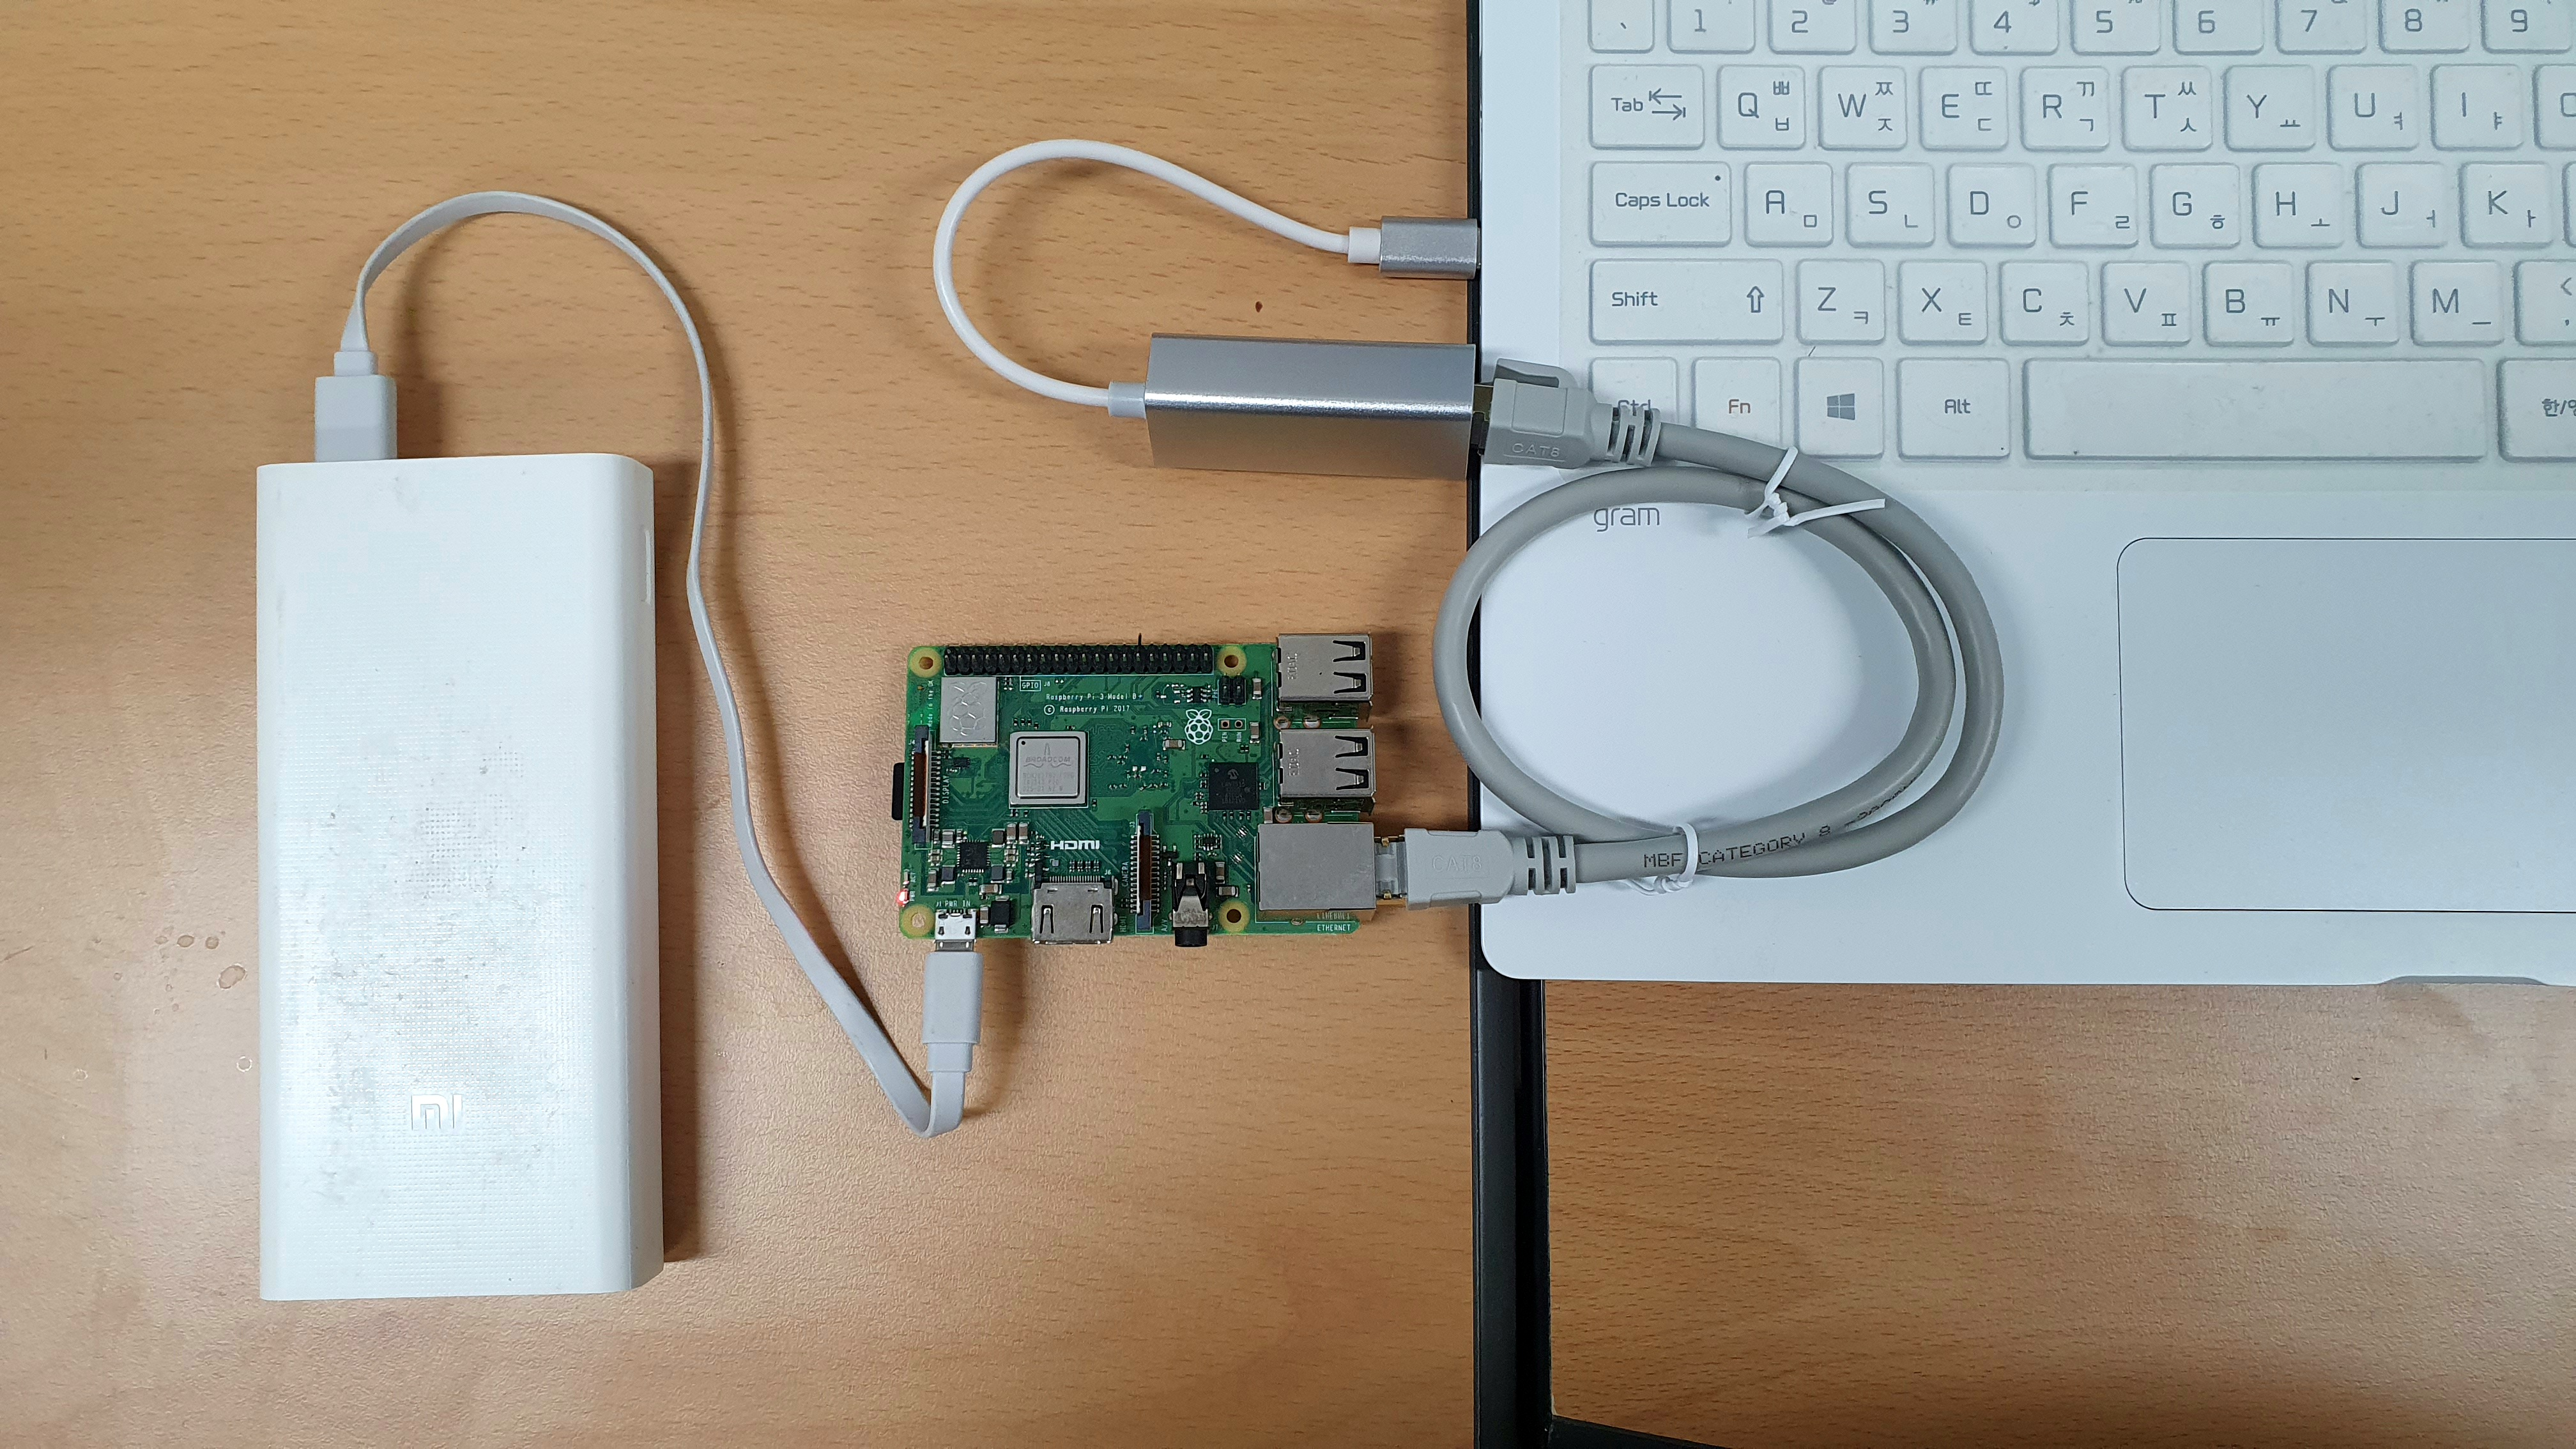
\includegraphics{content/material/ch2/connect-pi.jpg}

Step 5: Use PuTTY opeen putty remotely access the Pi using SSH (Secure
Shell), a protocol available on Linux systems that allows you to execute
commands on the Pi from your local computer. This method enables you to
access the Pi over an Ethernet cable, eliminating the need for a mouse
and monitor. SSH should be enabled during the Raspberry Pi OS
installation process (refer to Step 2).

\part{}

\hypertarget{section-2}{%
\chapter{}\label{section-2}}

\part{}

\hypertarget{section-4}{%
\chapter{}\label{section-4}}

\part{}

\hypertarget{section-6}{%
\chapter{}\label{section-6}}

\part{}

\url{image/access-1.mp4}

\hypertarget{section-8}{%
\chapter{}\label{section-8}}

\url{image/access-1.mp4}



\end{document}
